\documentclass[10pt, landscape]{article}
\usepackage[scaled=0.92]{helvet}
\usepackage{calc}
\usepackage{graphicx}
\usepackage{multicol}
\usepackage{ifthen}
\usepackage[a4paper,margin=3mm,landscape]{geometry}
\usepackage{amsmath,amsthm,amsfonts,amssymb}
\usepackage{color,graphicx,overpic}
\usepackage{hyperref}
\usepackage{newtxtext} 
\usepackage{enumitem}
\usepackage{graphicx}
\usepackage[table]{xcolor}
\usepackage{mathtools}
\usepackage[document]{ragged2e}
\usepackage{listings}
\setlist{nosep}
\usepackage{subfig}


% for including images
\graphicspath{ {./images/} }


\pdfinfo{
  /Title (CS3223.pdf)
  /Creator (TeX)
  /Producer (pdfTeX 1.40.0)
  /Author (Pei Cheng Yi)
  /Subject (CS3223)
  /Keywords (CS3223, nus,cheatsheet,pdf)}

% Turn off header and footer
\pagestyle{empty}

\newenvironment{tightcenter}{%
  \setlength\topsep{0pt}
  \setlength\parskip{0pt}
  \begin{center}
}{%
  \end{center}
}

% redefine section commands to use less space
\makeatletter
\renewcommand{\section}{\@startsection{section}{1}{0mm}%
                                {-1ex plus -.5ex minus -.2ex}%
                                {0.5ex plus .2ex}%x
                                {\normalfont\large\bfseries}}
\renewcommand{\subsection}{\@startsection{subsection}{2}{0mm}%
                                {-1explus -.5ex minus -.2ex}%
                                {0.5ex plus .2ex}%
                                {\normalfont\normalsize\bfseries}}
\renewcommand{\subsubsection}{\@startsection{subsubsection}{3}{0mm}%
                                {-1ex plus -.5ex minus -.2ex}%
                                {1ex plus .2ex}%
                                {\normalfont\small\bfseries}}%
\renewcommand{\familydefault}{\sfdefault}
\renewcommand\rmdefault{\sfdefault}
%  makes nested numbering (e.g. 1.1.1, 1.1.2, etc)
\renewcommand{\labelenumii}{\theenumii}
\renewcommand{\theenumii}{\theenumi.\arabic{enumii}.}
\renewcommand\labelitemii{•}
\renewcommand\labelitemiii{•}
%  convenient absolute value symbol
\newcommand{\abs}[1]{\vert #1 \vert}
%  convenient floor and ceiling
\newcommand{\floor}[1]{\lfloor #1 \rfloor}
\newcommand{\ceil}[1]{\lceil #1 \rceil}
%  convenient modulo
\newcommand{\Mod}[1]{\ \mathrm{mod}\ #1}
%  for logical not operator, iff symbol, convenient "if/then"
\renewcommand{\lnot}{\mathord{\sim}}
\let\then\Rightarrow
\let\Then\Rightarrow
%  vectors
\newcommand{\vv}[1]{\boldsymbol{#1}}
\newcommand{\VV}[1]{\overrightarrow{#1}}
%  column vector
\newcommand{\cvv}[1]{\left(\begin{smallmatrix}#1\end{smallmatrix}\right)}
\newcommand{\code}[1]{\textcolor{myblue}{\texttt{#1}}}
\newcommand\bggreen{\cellcolor{green!10}}

\makeatother
\definecolor{myblue}{cmyk}{1,.72,0,.38}
\everymath\expandafter{\the\everymath \color{myblue}}
% Define BibTeX command
\def\BibTeX{{\rm B\kern-.05em{\sc i\kern-.025em b}\kern-.08em
    T\kern-.1667em\lower.7ex\hbox{E}\kern-.125emX}}

% Don't print section numbers
\setcounter{secnumdepth}{0}

\setlength{\parindent}{0pt}
\setlength{\parskip}{0pt plus 0.5ex}
%% this changes all items (enumerate and itemize)
\setlength{\leftmargini}{0.5cm}
\setlength{\leftmarginii}{0.4cm}
\setlength{\leftmarginiii}{0.5cm}
\setlist[enumerate,1]{leftmargin=2mm,labelindent=1mm,labelsep=1mm}
\setlist[itemize,1]{leftmargin=2mm,labelindent=1mm,labelsep=1mm}
\setlist[itemize,2]{leftmargin=3mm,labelindent=1mm,labelsep=1mm}
\setlist[itemize,3]{leftmargin=3mm,labelindent=1mm,labelsep=1mm}

%My Environments
\newtheorem{example}[section]{Example}
% -----------------------------------------------------------------------

\begin{document}
\raggedright
\footnotesize
\begin{multicols}{4}


% multicol parameters
% These lengths are set only within the two main columns
\setlength{\columnseprule}{0.25pt}
\setlength{\premulticols}{1pt}
\setlength{\postmulticols}{1pt}
\setlength{\multicolsep}{1pt}
\setlength{\columnsep}{2pt}

\begin{center}
    \fbox{%
        \parbox{0.8\linewidth}{\centering \textcolor{black}{
            {\Large\textbf{CS3223}}
            \\ \normalsize{AY22/23 Sem 2}}
            \\ {\footnotesize \textcolor{myblue}{github.com/SeekSaveServe}}
        }%
    }
\end{center}

\section{L1 - Data Storage}
\subsection{Magnetic Disks}

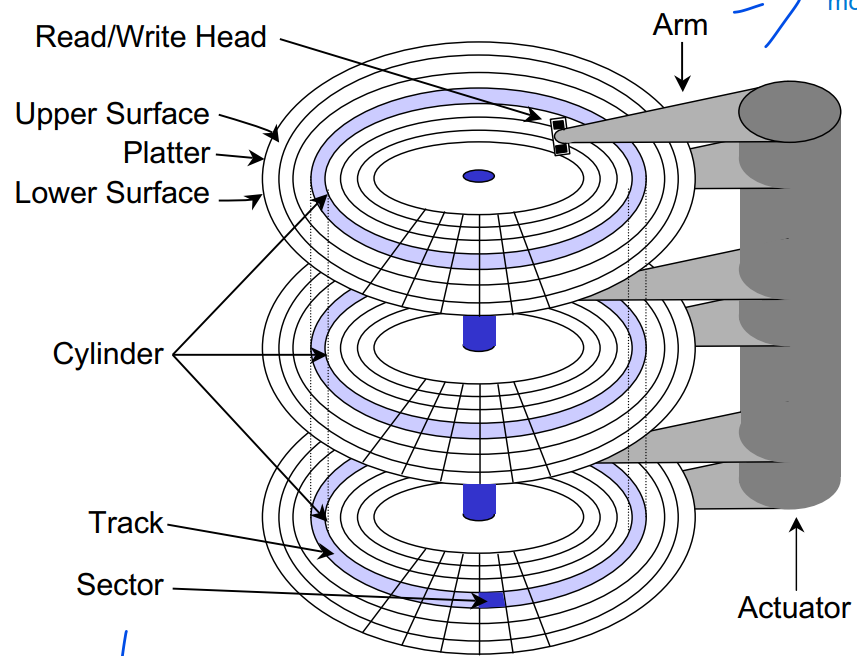
\includegraphics[width=3.5cm, height =2cm]{magnetic_disk.png}

\begin{itemize}
    \item \textbf{Disk Access Time} Seek time + Rotational Latency + Transfer time
    \item \textbf{Response time} Queueing delay + Disk access time
    \item \textbf{Rotational Delay} $\frac{1}{2} \frac{60s}{RPM}$ 
    \item \textbf{Transfer Time} sectors on the same track * $\tfrac{Time Per Revolution}{Sectors Per Track}$
\end{itemize}

\subsection{Buffer Manager}
\begin{itemize}
  \item \textbf{Buffer pool} Main memory allocated for DBMS
  \item \textbf{pin count} is incremented upon pinning
  \item \textbf{dirty bit} is updated when the page is unpinned (if modified)
  \item \textbf Replacement is only possbile if pin count == 0 
\end{itemize}

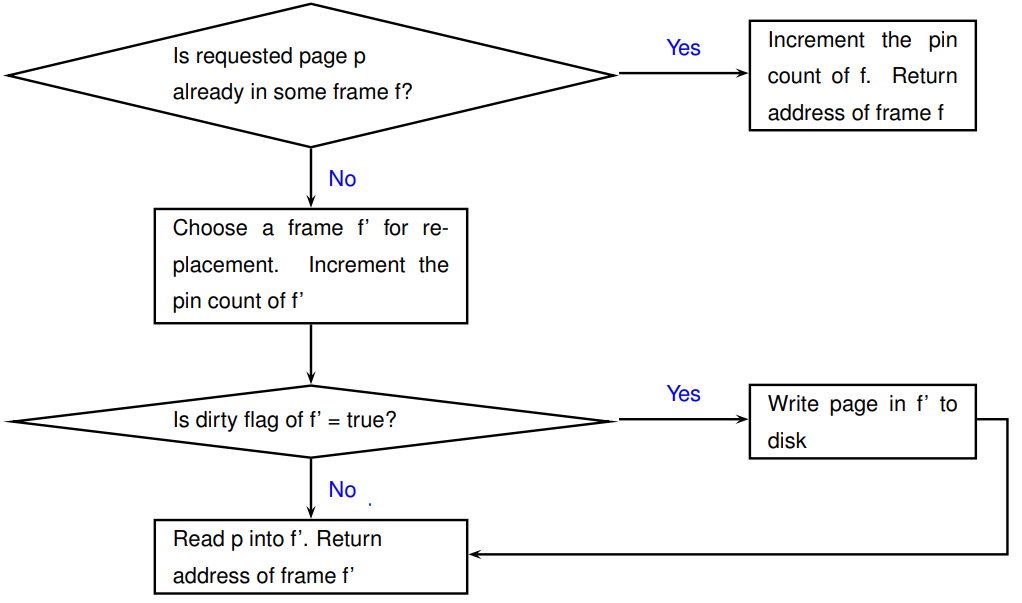
\includegraphics[width=5cm, height =3.5cm]{buff_manager_handle_request.png}

\subsection{Replacement Policies}
\textbf{LRU Policy}
\begin{itemize}
  \item Maintains a queue of pointers to frames with pin count = 0
\end{itemize}


\textbf{Clock Replacement Policy}
\includegraphics*[width=5cm, height=3.5cm]{clock.png}
\begin{itemize}
  \item Simplifies LRU with a second chance round robin system
  \item Each frame has a \textcolor{red}{reference bit} that is turned on when pin count reaches 0
  \item Repalces a page when referenced bit if off and pin count is 0
\end{itemize}

\subsection{File Organisation}
\includegraphics*[width=7cm, height=4cm]{heap_file.png}

\textbf{Page Formats: Fixed Length Records}
\begin{itemize}
  \item \textbf{Packed Organisation} Store records in contiguous slots
  \item \textbf{Unpacked Organisation} Uses a bit array to maintain free slots
\end{itemize}

\includegraphics*[width=7cm, height=4cm]{page_org.png}


\textbf{Page Formats: Slotted Page (variable length record)}
\begin{itemize}
  \item Store records in slots of \textsl{(record offset, record length)}
  \item Record Offset: Offset of the record from the start of the page
\end{itemize}

\includegraphics*[width=7cm, height=4cm]{slot_page.png}

\textbf{Record Formats}
\begin{itemize}
  \item 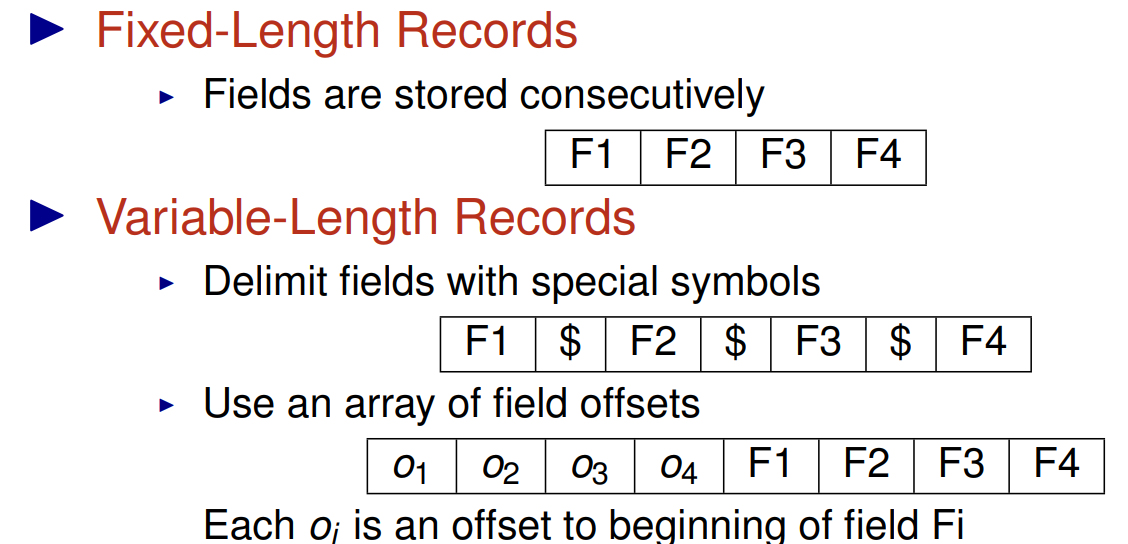
\includegraphics[width=3.5cm, height=2cm]{var_record.png}
\end{itemize}



\end{multicols}
\end{document}